

\usetikzlibrary{positioning,arrows.meta,quotes}
\usetikzlibrary{shapes,snakes}
\usetikzlibrary{bayesnet}
\tikzset{>=latex}


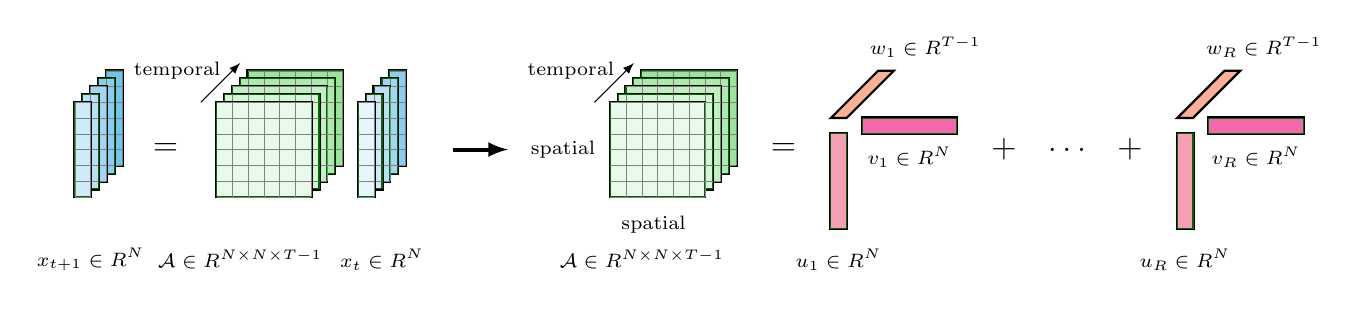
\begin{tikzpicture}
    
    % MF 
    % \draw (-1,1.2) node {\textbf{MF}};
    % \draw [very thick] (0,0+0.6) rectangle (3.6/2,0.6+2.4/2);
    % \filldraw [fill=Cerulean!40!white,draw=green!40!black] (0,0+0.6) rectangle (3.6/2,0.6+2.4/2);
    % \filldraw [fill=yellow!30] (0.4/2,0.6+0.4/2) rectangle (0.8/2,0.6+0.8/2);
    % \filldraw [fill=yellow!20] (2.4/2,0.6+0.4/2) rectangle (2.8/2,0.6+0.8/2);
    % \filldraw [fill=yellow!40] (0.8/2,0.6+1.2/2) rectangle (1.2/2,0.6+1.6/2);
    % \filldraw [fill=yellow!30] (2.0/2,0.6+1.6/2) rectangle (2.4/2,0.6+2.0/2);
    % \filldraw [fill=yellow!50] (0.4/2,0.6+2.0/2) rectangle (0.8/2,0.6+2.4/2);
    % \filldraw [fill=yellow!10] (2.4/2,0.6+2.0/2) rectangle (2.8/2,0.6+2.4/2);
    % \filldraw [fill=yellow!20] (2.8/2,0.6+1.2/2) rectangle (3.2/2,0.6+2.0/2);
    % \draw [step=0.4/2, very thin, color=gray] (0,0.6) grid (3.6/2,0.6+2.4/2);
    % \draw (1.8/2,-0.3+0.6) node {{\color{black}\scriptsize{$X\in\mathbb{R}^{N\times T}$}}};
    
    % % U
    % \draw (4.4/2,1.2/2+0.6) node {{\color{black}\large{$\approx$}}};
    % \draw [very thick] (5.2/2,0+0.6) rectangle (6.0/2,2.4/2+0.6);
    % \filldraw [fill=JungleGreen!30!white,draw=green!40!black] (5.2/2,0+0.6) rectangle (6.0/2,2.4/2+0.6);
    % \draw [step=0.4/2, very thin, color=gray] (5.2/2,0+0.6) grid (6.0/2,2.4/2+0.6);
    % \draw (5.6/2,-0.3+0.6) node {{\color{black}\scriptsize{$U\in\mathbb{R}^{N\times R}$}}};
    
    % % V
    % \draw (6.8/2,1.2/2+0.6) node {{\color{black}\large{$\times$}}};
    % \draw [very thick] (7.6/2,0.8/2+0.6) rectangle (11.2/2,1.6/2+0.6);
    % \filldraw [fill=blue!10!white,draw=blue!40!black] (7.6/2,0.8/2+0.6) rectangle (11.2/2,1.6/2+0.6);
    % \draw [step=0.4/2, very thin, color=gray] (7.6/2,0.8/2+0.6) grid (11.2/2,1.6/2+0.6);
    % \draw (9.4/2,0+0.6) node {{\color{black}\scriptsize{$V^{T}\in\mathbb{R}^{R\times T}$}}};
    
    % TVART MODEL
    % \draw (-1,-3.2) node {\textbf{TVART}};
    % t = 1
    % \draw [very thick] (0,-2.2) rectangle (0.2,-1);
    % \filldraw [fill=Cerulean!40!white,draw=green!40!black] (0,-2.2) rectangle (0.2,-1);
    % \filldraw [fill=yellow!50] (0,-1.2) rectangle (0.2,-1);
    % \filldraw [fill=yellow!30] (0,-2) rectangle (0.2,-1.8);
    % \draw [step=0.4/2, very thin, color=gray] (0,-2.2) grid (0.2,-1);
    % \draw (0.6,-1.6) node {{\color{black}\large{$\approx$}}};
    % \draw (0.2,-2.5) node {{\color{black}\scriptsize{$Y_1\in\mathbb{R}^{N}$}}};
    
    % \draw [very thick] (1,-2.2) rectangle (2.2,-1);
    % \filldraw [fill=LimeGreen!40!white,draw=green!40!black] (1,-2.2) rectangle (2.2,-1);
    % \draw [step=0.4/2, very thin, color=gray] (1,-2.2) grid (2.2,-1);
    % \draw (1.6,-2.5) node {{\color{black}\scriptsize{$A_1\in\mathbb{R}^{N \times N}$}}};
    
    % \draw (2.6,-1.6) node {{\color{black}\large{$\times$}}};
    % \draw [very thick] (3,-2.2) rectangle (3.2,-1);
    % \filldraw [fill=Cerulean!40!white,draw=green!40!black] (3,-2.2) rectangle (3.2,-1);
    % \draw [step=0.4/2, very thin, color=gray] (3,-2.2) grid (3.2,-1);
    % \draw (3.2,-2.5) node {{\color{black}\scriptsize{$X_1\in\mathbb{R}^{N}$}}};
    
    % \draw (1.6,-3.2) node {{\color{black}\large{$\dots$}}};
    
    % % t = T
    % \draw [very thick] (0,-2.2-3+0.2) rectangle (0.2,-1-3+0.2);
    % \filldraw [fill=Cerulean!40!white,draw=green!40!black] (0,-2.2-3+0.2) rectangle (0.2,-1-3+0.2);
    % \draw [step=0.4/2, very thin, color=gray] (0,-2.2-3+0.2) grid (0.2,-1-3+0.2);
    % \draw (0.6,-1.6-3+0.2) node {{\color{black}\large{$\approx$}}};
    % \draw (0.2,-2.5-3+0.2) node {{\color{black}\scriptsize{$Y_T\in\mathbb{R}^{N}$}}};
    
    % \draw [very thick] (1,-2.2-3+0.2) rectangle (2.2,-1-3+0.2);
    % \filldraw [fill=LimeGreen!40!white,draw=green!40!black] (1,-2.2-3+0.2) rectangle (2.2,-1-3+0.2);
    % \draw [step=0.4/2, very thin, color=gray] (1,-2.2-3+0.2) grid (2.2,-1-3+0.2);
    % \draw (1.6,-2.5-3+0.2) node {{\color{black}\scriptsize{$A_T\in\mathbb{R}^{N \times N}$}}};
    
    % \draw (2.6,-1.6-3+0.2) node {{\color{black}\large{$\times$}}};
    % \draw [very thick] (3,-2.2-3+0.2) rectangle (3.2,-1-3+0.2);
    % \filldraw [fill=Cerulean!40!white,draw=green!40!black] (3,-2.2-3+0.2) rectangle (3.2,-1-3+0.2);
    % \filldraw [fill=yellow!20] (3,-4.2) rectangle (3.2,-4);
    % \filldraw [fill=yellow!20] (3,-4.4) rectangle (3.2,-4.2);
    % \draw [step=0.4/2, very thin, color=gray] (3,-2.2-3+0.2) grid (3.2,-1-3+0.2);
    % \draw (3.2,-2.5-3+0.2) node {{\color{black}\scriptsize{$X_T\in\mathbb{R}^{N}$}}};
    
    
    % AR MODEL
    \draw [very thick] (.8+0.4,-3.8+0.4) rectangle (2+0.4,-2.6+0.4);
    \filldraw [fill=LimeGreen!50!white,draw=green!40!black] (.8+0.4,-3.8+0.4) rectangle (2+0.4,-2.6+0.4);
    \draw [step=0.4/2, very thin, color=gray] (.8+0.4,-3.8+0.4) grid (2+0.4,-2.6+0.4);
    
    \draw [very thick] (.8+0.3,-3.8+0.3) rectangle (2+0.3,-2.6+0.3);
    \filldraw [fill=LimeGreen!40!white,draw=green!40!black] (.8+0.3,-3.8+0.3) rectangle (2+0.3,-2.6+0.3);
    \draw [step=0.4/2, very thin, color=gray] (.8+0.3,-3.8+0.3) grid (2+0.3,-2.6+0.3);
    
    \draw [very thick] (.8+0.2,-3.8+0.2) rectangle (2+0.2,-2.6+0.2);
    \filldraw [fill=LimeGreen!30!white,draw=green!40!black] (.8+0.2,-3.8+0.2) rectangle (2+0.2,-2.6+0.2);
    \draw [step=0.4/2, very thin, color=gray] (.8+0.2,-3.8+0.2) grid (2+0.2,-2.6+0.2);
    
    \draw [very thick] (.8+0.1,-3.8+0.1) rectangle (2+0.1,-2.6+0.1);
    \filldraw [fill=LimeGreen!20!white,draw=green!40!black] (.8+0.1,-3.8+0.1) rectangle (2+0.1,-2.6+0.1);
    \draw [step=0.4/2, very thin, color=gray] (.8+0.1,-3.8+0.1) grid (2+0.1,-2.6+0.1);
    
    \draw [very thick] (.8,-3.8) rectangle (2,-2.6);
    \filldraw [fill=LimeGreen!10!white,draw=green!40!black] (.8,-3.8) rectangle (2,-2.6);
    \draw [step=0.4/2, very thin, color=gray] (.8,-3.8) grid (2,-2.6);
    
      \draw (1.1,-4.6) node
    {{\color{black}\scriptsize{$\mathcal{A}\in\mathbb{R}^{N \times N \times T-1}$}}};
    % y vector

    \draw [very thick] (0+0.4-0.8-0.2,-3.8+0.4) rectangle (0.2+0.4-0.8-0.2,-2.6+0.4);
    \filldraw [fill=Cerulean!60!white,draw=green!40!black] (0+0.4-0.8-0.2,-3.8+0.4) rectangle (0.2+0.4-0.8-0.2,-2.6+0.4);
    \draw [step=0.4/2, very thin, color=gray] (0+0.4-0.8-0.2,-3.8+0.4) grid (0.2+0.4-0.8-0.2,-2.6+0.4);
    
    \draw [very thick] (0+0.3-0.8-0.2,-3.8+0.3) rectangle (0.2+0.3-0.8-0.2,-2.6+0.3);
    \filldraw [fill=Cerulean!50!white,draw=green!40!black] (0+0.3-0.8-0.2,-3.8+0.3) rectangle (0.2+0.3-0.8-0.2,-2.6+0.3);
    \draw [step=0.4/2, very thin, color=gray] (0+0.3-0.8-0.2,-3.8+0.3) grid (0.2+0.3-0.8-0.2,-2.6+0.3);

    \draw [very thick] (0+0.2-0.8-0.2,-3.8+0.2) rectangle (0.2+0.2-0.8-0.2,-2.6+0.2);
    \filldraw [fill=Cerulean!40!white,draw=green!40!black] (0+0.2-0.8-0.2,-3.8+0.2) rectangle (0.2+0.2-0.8-0.2,-2.6+0.2);
    \draw [step=0.4/2, very thin, color=gray] (0+0.2-0.8-0.2,-3.8+0.2) grid (0.2+0.2-0.8-0.2,-2.6+0.2);
    
    \draw [very thick] (0.1-0.8-0.2,-3.8+0.1) rectangle (0.2+0.1-0.8-0.2,-2.6+0.1);
    \filldraw [fill=Cerulean!30!white,draw=green!40!black] (0+0.1-0.8-0.2,-3.8+0.1) rectangle (0.2+0.1-0.8-0.2,-2.6+0.1);
    \draw [step=0.4/2, very thin, color=gray] (0+0.1-0.8-0.2,-3.8+0.1) grid (0.2+0.1-0.8-0.2,-2.6+0.1);
    
    \draw [very thick] (0-0.8-0.2,-3.8) rectangle (0.2-0.8-0.2,-2.6);
    \filldraw [fill=Cerulean!20!white,draw=green!40!black] (0-0.8-0.2,-3.8) rectangle (0.2-0.8-0.2,-2.6);
    \draw [step=0.4/2, very thin, color=gray] (0-0.8-0.2,-3.8) grid (0.2-0.8-0.2,-2.6);
     \draw (0-0.8,-4.6) node {{\color{black}\scriptsize{$\boldsymbol{x}_{t+1}\in\mathbb{R}^{N}$}}};
    
     \draw (0.15,-3.2) node {{\color{black}\large{$=$}}};
    % x vector
    \draw [very thick] (0+0.4+2.6,-3.8+0.4) rectangle (0.2+0.4+2.6,-2.6+0.4);
    \filldraw [fill=Cerulean!50!white,draw=green!40!black] (0+0.4+2.6,-3.8+0.4) rectangle (0.2+0.4+2.6,-2.6+0.4);
    \draw [step=0.4/2, very thin, color=gray] (0+0.4+2.6,-3.8+0.4) grid (0.2+0.4+2.6,-2.6+0.4);
    
    \draw [very thick] (0+0.3+2.6,-3.8+0.3) rectangle (0.2+0.3+2.6,-2.6+0.3);
    \filldraw [fill=Cerulean!40!white,draw=green!40!black] (0+0.3+2.6,-3.8+0.3) rectangle (0.2+0.3+2.6,-2.6+0.3);
    \draw [step=0.4/2, very thin, color=gray] (0+0.3+2.6,-3.8+0.3) grid (0.2+0.3+2.6,-2.6+0.3);

    \draw [very thick] (0+0.2+2.6,-3.8+0.2) rectangle (0.2+0.2+2.6,-2.6+0.2);
    \filldraw [fill=Cerulean!30!white,draw=green!40!black] (0+0.2+2.6,-3.8+0.2) rectangle (0.2+0.2+2.6,-2.6+0.2);
    \draw [step=0.4/2, very thin, color=gray] (0+0.2+2.6,-3.8+0.2) grid (0.2+0.2+2.6,-2.6+0.2);
    
    \draw [very thick] (0.1+2.6,-3.8+0.1) rectangle (0.2+0.1+2.6,-2.6+0.1);
    \filldraw [fill=Cerulean!20!white,draw=green!40!black] (0+0.1+2.6,-3.8+0.1) rectangle (0.2+0.1+2.6,-2.6+0.1);
    \draw [step=0.4/2, very thin, color=gray] (0+0.1+2.6,-3.8+0.1) grid (0.2+0.1+2.6,-2.6+0.1);
    
    \draw [very thick] (0+2.6,-3.8) rectangle (0.2+2.6,-2.6);
    \filldraw [fill=Cerulean!10!white,draw=green!40!black] (0+2.6,-3.8) rectangle (0.2+2.6,-2.6);
    \draw [step=0.4/2, very thin, color=gray] (0+2.6,-3.8) grid (0.2+2.6,-2.6);
    
    \draw (2.9 ,-4.6) node {{\color{black}\scriptsize{$\boldsymbol{x}_{t}\in\mathbb{R}^{N}$}}};

    \draw[->] (0.6,-2.6) -- (1.1,-2.1);
    \draw (0.3,-2.2) node {{\color{black}\scriptsize{temporal}}};

    \draw[->, line width=0.5mm] (3.8,-3.2) -- (4.5,-3.2);
    
    % tensor A
    \draw [very thick] (5.8+0.4,-3.8+0.4) rectangle (7+0.4,-2.6+0.4);
    \filldraw [fill=LimeGreen!50!white,draw=green!40!black] (5.8+0.4,-3.8+0.4) rectangle (7+0.4,-2.6+0.4);
    \draw [step=0.4/2, very thin, color=gray] (5.8+0.4,-3.8+0.4) grid (7+0.4,-2.6+0.4);
    
    \draw [very thick] (5.8+0.3,-3.8+0.3) rectangle (7+0.3,-2.6+0.3);
    \filldraw [fill=LimeGreen!40!white,draw=green!40!black] (5.8+0.3,-3.8+0.3) rectangle (7+0.3,-2.6+0.3);
    \draw [step=0.4/2, very thin, color=gray] (5.8+0.3,-3.8+0.3) grid (7+0.3,-2.6+0.3);
    
    \draw [very thick] (5.8+0.2,-3.8+0.2) rectangle (7+0.2,-2.6+0.2);
    \filldraw [fill=LimeGreen!30!white,draw=green!40!black] (5.8+0.2,-3.8+0.2) rectangle (7+0.2,-2.6+0.2);
    \draw [step=0.4/2, very thin, color=gray] (5.8+0.2,-3.8+0.2) grid (7+0.2,-2.6+0.2);
    
    \draw [very thick] (5.8+0.1,-3.8+0.1) rectangle (7+0.1,-2.6+0.1);
    \filldraw [fill=LimeGreen!20!white,draw=green!40!black] (5.8+0.1,-3.8+0.1) rectangle (7+0.1,-2.6+0.1);
    \draw [step=0.4/2, very thin, color=gray] (5.8+0.1,-3.8+0.1) grid (7+0.1,-2.6+0.1);
    
    \draw [very thick] (5.8,-3.8) rectangle (7,-2.6);
    \filldraw [fill=LimeGreen!10!white,draw=green!40!black] (5.8,-3.8) rectangle (7,-2.6);
    \draw [step=0.4/2, very thin, color=gray] (5.8,-3.8) grid (7,-2.6);
   % 
   % \draw[->] (5.8,-4) -- (7,-4);
   % \draw[->] (5.6,-3.8) -- (5.6,-2.7);
    \draw[->] (5.6,-2.6) -- (6.1,-2.1);
    
    \draw (6.35,-4.15) node {{\color{black}\scriptsize{spatial}}};
    \draw (5.2,-3.2) node {{\color{black}\scriptsize{spatial}}};
    \draw (5.3,-2.2) node {{\color{black}\scriptsize{temporal}}};
    
    \draw (6.2,-4.6) node {{\color{black}\scriptsize{$\mathcal{A}\in\mathbb{R}^{N \times N \times T-1}$}}};
  
    \draw (8,-3.2) node {{\color{black}\large{$=$}}};

    % CP 
    \draw [very thick] (8.6,-4.4+0.2) rectangle (8.8,-3.2+0.2);
    \filldraw [fill=WildStrawberry!40!white,draw=green!40!black] (8.6,-4.4+0.2) rectangle (8.8,-3.2+0.2);
    %\draw [step=0.4/2, very thin, color=gray] (8.6,-4.4) grid (8.8,-3.2);
    \draw (8.7,-4.8+0.2) node {{\color{black}\scriptsize{$\boldsymbol{u}_1 \in \mathbb{R}^N$}}};
    
    \draw [very thick] (9,-3-0.2+0.2) rectangle (10.2,-2.8-0.2+0.2);
    \filldraw [fill=RubineRed!60!white,draw=green!40!black] (9,-3-0.2+0.2) rectangle (10.2,-2.8-0.2+0.2);
    %\draw [step=0.2, very thin, color=gray] (9,-3-0.2) grid (10.2,-2.8-0.2);
    \draw (9.6,-3.3-0.2+0.2) node {{\color{black}\scriptsize{$\boldsymbol{v}_1 \in \mathbb{R}^N$}}};
    
    %\draw [very thick] (8.6,-2.6) rectangle (8.8,-1.8);
    \draw[fill=RedOrange!40!white, line width=0.8pt] (9.2,-2.4+0.2) -- (9.4,-2.4+0.2) -- (8.8,-3+0.2) -- (8.6,-3+0.2) -- cycle;
   % \draw [step=0.2, very thin, color=gray] (9.2,-2.4) -- (9.4,-2.4) -- (8.8,-3) -- (8.6,-3) -- cycle;
    %\filldraw [fill=RedOrange!40!white,draw=green!40!black,rotate around={-45:(8.6,-2.6)}] (8.6,-2.6) rectangle (8.8,-1.8);
    %\draw [step=0.2, very thin, color=gray,rotate around={-45:(8.6,-2.6)}] (8.6,-2.6) grid (8.8,-1.8);
    \draw (10-0.2,-1.9) node {{\color{black}\scriptsize{$\boldsymbol{w}_1 \in \mathbb{R}^{T-1}$}}};

    \draw (10.8,-3.2) node {{\color{black}\large{$+$}}};
    \draw (11.6,-3.2) node {{\color{black}\large{$\dots$}}};
    \draw (12.4,-3.2) node {{\color{black}\large{$+$}}};
    
    \draw [very thick] (8.6+4.4,-4.4+0.2) rectangle (8.8+4.4,-3.2+0.2);
    \filldraw [fill=WildStrawberry!40!white,draw=green!40!black] (8.6+4.4,-4.4+0.2) rectangle (8.8+4.4,-3.2+0.2);
    %\draw [step=0.4/2, very thin, color=gray] (8.6+4.4,-4.4) grid (8.8+4.4,-3.2);
    \draw (8.7+4.4,-4.8+0.2) node {{\color{black}\scriptsize{$\boldsymbol{u}_R \in \mathbb{R}^N $}}};
    
    \draw [very thick] (9+4.4,-3-0.2+0.2) rectangle (10.2+4.4,-2.8-0.2+0.2);
    \filldraw [fill=RubineRed!60!white,draw=green!40!black] (9+4.4,-3-0.2+0.2) rectangle (10.2+4.4,-2.8-0.2+0.2);
    %\draw [step=0.2, very thin, color=gray] (9+4.4,-3) grid (10.2+4.4,-2.8);
    \draw (9.6+4.4,-3.3-0.2+0.2) node {{\color{black}\scriptsize{$\boldsymbol{v}_R\in \mathbb{R}^N$}}};
    
    \draw[fill=RedOrange!40!white, line width=0.8pt] (9.2+4.4,-2.4+0.2) -- (9.4+4.4,-2.4+0.2) -- (8.8+4.4,-3+0.2) -- (8.6+4.4,-3+0.2) -- cycle;
   % \draw [very thick] (8.6+4.4,-2.6) rectangle (8.8+4.4,-1.6);
   % \filldraw [fill=RedOrange!40!white,draw=green!40!black] (8.6+4.4,-2.6) rectangle (8.8+4.4,-1.6);
    %\draw [step=0.2, very thin, color=gray] (8.6+4.4,-2.6) grid (8.8+4.4,-1.6);
    \draw (10.1+4,-1.9) node {{\color{black}\scriptsize{$\boldsymbol{w}_R\in \mathbb{R}^{T-1}$}}};
    
\end{tikzpicture}
